\section{Objetivo del Proyecto}

El objetivo de la presente es determinar si el cuidado de plantas automatizado con robótica es: eficiente, escalable y sostenible a largo plazo. De este modo, se espera que Agrocare pueda ser utilizado para medir los valores que afectan el crecimiento de una planta, que incluyen humedad del suelo, humedad relativa, luz solar y temperatura, posteriormente, estos datos serán analizados en un servidor remoto apoyándose de un microservicio de Red Neuronal Recurrente y una base de datos. Se espera que el flujo de datos sea el siguiente:

\renewcommand{\figurename}{Figura}
\begin{figure}[h]
  \centering
  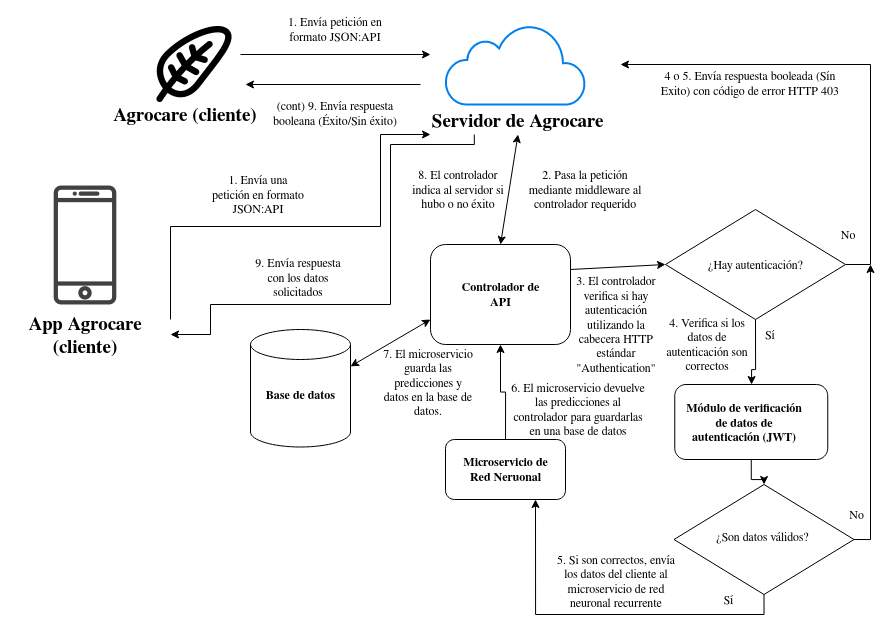
\includegraphics[width=\linewidth]{diagrama.png}
  \caption{Diagrama del flujo de datos}
  \label{fig:example}
\end{figure}

Una vez obtenidos estos datos, se podrá demostrar con datos estadísticos la efectividad de la robótica en la agricultura, que da pie a la posterior utilización de estos sistemas en producción.